\section{Aerodynamics}
\label{sec:aero}

\path{Aerodynamics.py} returns Body-frame forces and CG moments using the evidence-qualified register \path{data/aero_configurations.json}. Four configurations serve stack/booster phases; a fifth, \texttt{second\_stack}, is declared but not selected by the independent upper-stage drag provider (Section~\ref{sec:mission-exec}).

\subsection{Flow state and force build-up}

Equation~\eqref{eq:aero-flow} defines the relative flow and total angle:
%
\begin{equation}
\label{eq:aero-flow}
\mathbf{v}_{\mathrm{rel}} = \mathbf{v}_{\mathrm{CG}}
- \dot{\mathbf{c}} - \mathbf{w},
\qquad
\alpha = \operatorname{atan2}\bigl(\, \lVert \mathbf{v}_{\mathrm{rel},yz}\rVert, \; v_{\mathrm{rel},x} \,\bigr),
\end{equation}
%
where $\dot{\mathbf{c}}$ is the axial center-of-gravity migration rate
(Section~\ref{sec:vehicle}, stage depletion) and $\mathbf{w}$ the wind in
Body components (Section~\ref{sec:environment}). The total flow angle
$\alpha$ spans $0$ (nose-first) to $\pi$ (engine-first); every direction in
the lateral plane is handled, not only a pitch plane. The dynamic pressure
is $\bar{q} = \tfrac{1}{2}\,\rho\,v_{\mathrm{rel}}^2$ with the atmosphere
state of Section~\ref{sec:environment}.

The axial and potential-normal loads follow Equation~\eqref{eq:aero-axial-normal}; side segments add the crossflow terms of Equation~\eqref{eq:aero-crossflow}:
%
\begin{equation}
\label{eq:aero-axial-normal}
F_x = -\,\bar{q}\, S_{\mathrm{ref}}\, CA_0(M)\,\cos\alpha
\,|\!\cos\alpha|,
\qquad
N = \bar{q}\, S_{\mathrm{ref}}\, C_{N\alpha}\, \sin\alpha
\,|\!\cos\alpha|,
\end{equation}
%
\begin{equation}
\label{eq:aero-crossflow}
D_i = \bar{q}\; C_{Dc,i}\, S_i \,\sin^2\alpha
\qquad \text{per side segment } i,
\end{equation}
%
Reference areas/lengths appear in Table~\ref{tab:aero-configurations}. Normal force opposes lateral flow at a windward-end station (57.6 m for the stack, 41.0 m for the booster), mirrored about CG for retro flow. Crossflow forces act at side-area centroids. The landing configuration adds fin and deployed-leg segments to the body model.

The $\cos\alpha|\cos\alpha|$ factor reverses the axial load and fixed-deflection fin effect in engine-first flight and makes them vanish at $90^\circ$. Station moments are assembled once as $(\vect s-\vect c)\times\vect F$. Geometry determines restoring or destabilizing effects; the model does not impose passive stability.

Equation~\eqref{eq:aero-damping} closes the moment set with per-axis damping:
%
\begin{equation}
\label{eq:aero-damping}
\mathbf{M}_{\mathrm{damp}} = \operatorname{diag}(c_l,c_m,c_m)\,
\frac{\bar{q}\, S_{\mathrm{ref}}\, L_{\mathrm{ref}}^2}{2\,v_{\mathrm{rel}}}
\;\boldsymbol{\omega},
\end{equation}
%
with pitch and yaw coefficient $c_m$ tied by symmetry and roll coefficient $c_l$ separate (declared values: $-10$ full stack, $-20$ booster, roll $-3$ with fins
deployed; a zero coefficient means that no roll-damping contribution is applied).

\subsection{Configurations and axial curves}

\par\medskip\noindent\begin{minipage}{\linewidth}
\centering
\begin{tabular}{llrrl}
\toprule
Configuration & Phase & $S_{\mathrm{ref}}$ [m$^2$] & $L_{\mathrm{ref}}$ [m] & Axial curve / fins \\
\midrule
\texttt{full\_stack} & launch to separation & 21.08 & 62.4 & sourced $M\,0$--$7$; declared $M\,7$--$10$ \\
\texttt{booster\_alone} & coast, boostback & 10.52 & 42.6 & declared ($\pm 50\,\%$) \\
\texttt{booster\_return} & entry burn, descent & 10.52 & 42.6 & declared; four fins \\
\texttt{booster\_landing} & landing burn & 10.52 & 42.6 & declared; four fins and legs \\
\texttt{second\_stack} & stage-2 body (declared) & 10.52 & 19.8 & declared, sleeker estimate \\
\bottomrule
\end{tabular}
\captionof{table}{The five aerodynamic configurations. Station datum is the
configuration's own structural base. Fins deploy after boostback; the legs
deploy at landing ignition, which is represented by the segment difference
between \texttt{booster\_return} and \texttt{booster\_landing}.}
\label{tab:aero-configurations}
\end{minipage}\par\medskip

Figure~\ref{fig:aero-axial-curves} shows the adopted $CA_0(M)$ curves. The full-stack curve to Mach 7 is read from Pezent's RasAeroII analysis of a Falcon-9-like stack with fairing \cite{pezent2024}; its transonic peak is about 1.16 near Mach 1.06. The extension to Mach 10 and all booster/upper curves are engineering estimates, with declared uncertainties around $\pm50\%$ for the unsourced curves. The fairing-stack curve is transferred to Dragon geometry as an E/A approximation: reference area and coefficient normalization must be retained together. It is not a CRS-10-specific aerodynamic identification.

\par\medskip\noindent\begin{minipage}{\linewidth}
\centering
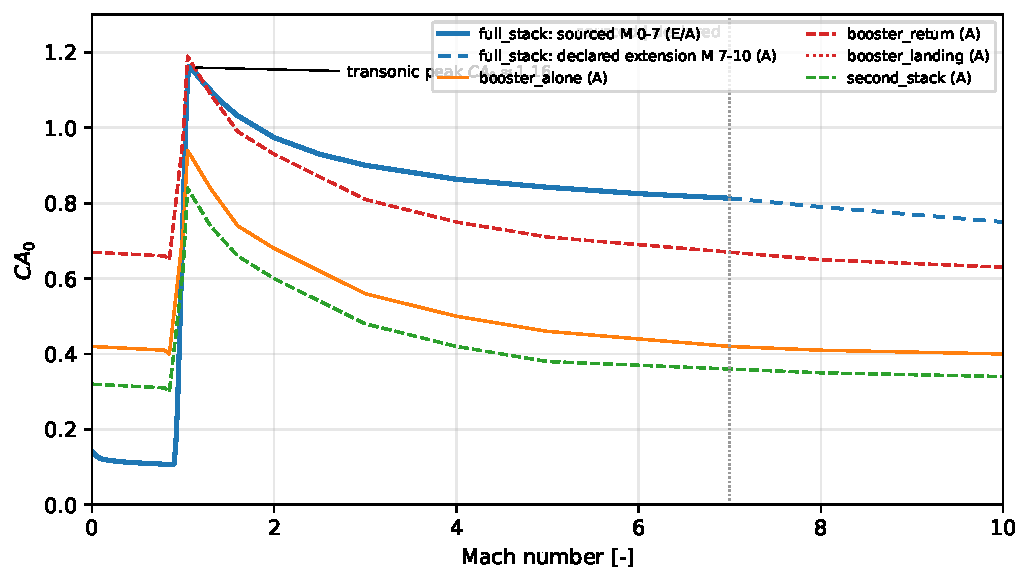
\includegraphics[width=0.85\linewidth]{images/aero_axial_curves.pdf}
\captionof{figure}{Axial drag coefficient $CA_0(M)$ of the five configurations.
Only the full-stack curve to Mach~7 is sourced; everything else is a
declared estimate (evidence classes in the legend). The transonic peak of
the full stack reaches $CA_0 \approx 1.16$.}
\label{fig:aero-axial-curves}
\end{minipage}\par\medskip

\subsection{Grid fin control}

The return/landing configurations have four fins at $45^\circ$, $135^\circ$, $225^\circ$ and $315^\circ$ about Body $+x$, station 39.6 m and pivot radius 1.83 m. Each uses area $1.65\,\mathrm{m^2}$, effective lift slope $1.2\,\mathrm{rad^{-1}}$ and travel $\pm0.35\,\mathrm{rad}$, all research-model assumptions. Equation~\eqref{eq:aero-fin} gives the force for deflection $\delta_i$ and azimuth $\varphi_i$:
\begin{equation}
 \vect F_i=\bar q S_{\mathrm{fin}}c_{\ell,\delta}\delta_i\cos\alpha|\cos\alpha|
 \begin{bmatrix}0&-\sin\varphi_i&\cos\varphi_i\end{bmatrix}^{\mathsf T}.
\label{eq:aero-fin}
\end{equation}
The three-dimensional mount arm generates pitch/yaw through axial offset and roll through radial offset. Equal deflections produce roll; differential pairs generate transverse moments. Command selection belongs to Section~\ref{sec:mission-exec}. The aerodynamic interface applies instantaneous deflections without servo dynamics. Mach/angle-dependent effectiveness, plume interference and deflection-induced axial drag are unresolved.

\subsection{Domain and verification}

The model rejects unsupported Mach values (the curves end at 10), unknown configurations, invalid stations and out-of-travel commands. Declared coefficient uncertainty remains an uncertainty within that domain, not an execution error.

The 42 aerodynamic tests check axial baselines, force direction, retro reversal, moment arms, dissipative damping, continuity, fin combinations and all configuration records, plus a short propagation through the dynamics provider. These checks verify the implementation; they do not validate the unsourced coefficient curves against flight data.
